\documentclass[11pt, a4paper]{article}

% 한글 폰트 설정을 위한 패키지 (XeLaTeX 또는 LuaLaTeX 컴파일 필요)
\usepackage{kotex}
% 사용자 지정 폰트 (동일 디렉토리에 Pretendard 폰트가 위치하거나 시스템에 설치되어 있어야 함)
\setmainhangulfont{Pretendard-Regular.ttf}[
    BoldFont=Pretendard-Bold.ttf,
    AutoFakeSlant=true
]
\setmainfont{Pretendard-Regular.ttf}[
    BoldFont=Pretendard-Bold.ttf,
    AutoFakeSlant=true
]

\usepackage{graphicx}
\usepackage{geometry}
\usepackage{hyperref}
\usepackage{float}
\usepackage[labelfont=bf]{caption}
\usepackage{setspace}
\setstretch{1.3}

\geometry{
    a4paper,
    total={170mm,240mm},
    left=20mm,
    top=20mm,
}

\renewenvironment{abstract}{%
  \begin{center}%
    {\Large\bfseries \abstractname\vspace{-0.5em}\vspace{\z}}%
  \end{center}%
  \quotation
  \normalsize
}{%
  \endquotation
}

\title{\textbf{Analysis of Lin28a Translational Repression Characteristics}}
\author{학번: 2025-25159 \\ 이름: 김보현}
\date{\today}

\begin{document}

\maketitle

\begin{abstract}
Lin28a는 발달 및 종양 형성에 중요한 역할을 하는 RNA 결합 단백질(RNA-binding protein)로서 표적 mRNA의 번역(Translation)을 억제한다고 알려져 있다. 본 보고서에서는 리보솜 프로파일링(Ribosome Profiling) 및 RNA-seq 데이터를 기반으로 Lin28a Knockdown 시 나타나는 번역 억제 해제(Derepression) 양상을 정량적으로 분석했다. 표적 mRNA에 대한 물리적 결합 강도(CLIP Enrichment)와 mRNA가 번역되는 세포 내 공간(Subcellular Localization)이 번역 억제 강도에 미치는 영향을 확인하였다. 분석 결과, Lin28a의 번역 억제 효과는 표적 RNA와의 결합 강도에 비례하는 용량 의존적 패턴(Graded Derepression)을 보이며, 동시에 Free Ribosome과 ER-bound Ribosome 간에 조절 방식이 상이할 수 있음을 시사한다.
\end{abstract}

\section{Introduction}
전사 후 조절(Post-transcriptional regulation)은 세포 내 유전자 발현을 환경에 맞추어 미세 조정하는 핵심적인 단계다. 특히 RNA 결합 단백질인 Lin28a는 초기 발생 과정 및 줄기세포의 다분화능(pluripotency) 유지에 필수적인 역할을 한다. 구조적으로 Lin28a는 두 개의 RNA 결합 도메인인 Cold Shock Domain(CSD)과 두 개의 CCHC-type zinc finger 도메인을 포함하고 있으며, 이를 통해 표적 RNA의 특정 서열(특히 GGAG 모티프)에 높은 친화도로 직접 결합한다. Lin28a는 일차적으로 let-7 마이크로RNA의 전구체(pre-let-7)에 결합하여 말단 유리딜화(terminal uridylation)를 유도함으로써 그 성숙을 억제하고 세포 분화를 막는 역할로 잘 알려져 있다 \cite{heo2008}. 그러나 최근 연구에 따르면, Lin28a는 let-7 종속적 경로 외에도 다수의 mRNA에 직접 결합하여 이들의 번역 효율(Translation Efficiency, TE)을 조절하는 전반적인 전사 후 조절 인자로서 작용함이 밝혀졌다 \cite{hu2024}.

이러한 유전자 발현 조절을 정량적으로 분석하기 위해, 전사체 분석(RNA-seq)과 리보솜 프로파일링(Ribosome Profiling) 기술의 결합이 널리 활용된다. RNA-seq은 세포 내에 존재하는 전체 mRNA의 양을 측정하는 반면, 리보솜 프로파일링은 실제로 번역이 진행 중인 리보솜이 보호하고 있는 mRNA 단편(Ribosome Protected Fragments, RPF)만을 시퀀싱한다. 따라서 특정 유전자의 RPF 양을 RNA-seq 양으로 정규화한 값인 번역 효율(TE = RPF / RNA-seq)을 산출함으로써, Translation 단계에서의 조절 강도를 정밀하게 측정할 수 있다.

특히 Cho et al. (2012)의 연구에서는 CLIP-seq 및 리보솜 프로파일링 기법을 통해 Lin28a가 주로 소포체(Endoplasmic Reticulum, ER) 주변에 국소화되어 분비 경로(secretory pathway)로 향하는 표적 mRNA의 번역을 선택적으로 억제한다는 것을 증명하였다 \cite{cho2012}. 이러한 배경을 바탕으로, 억제의 강도가 mRNA의 물리화학적 결합 특성이나 공간적 특성에 어떻게 의존하는지를 보다 구체적으로 확인할 필요성이 제기된다. 단순히 결합 유무만을 따지는 이분법적인 분석을 넘어, 결합 강도의 세기와 번역이 일어나는 실제 미세환경(microenvironment)의 공간적 맥락에 따라 번역 제어가 어떻게 차등화(graded)되는지 정량적인 검증이 요구된다.

본 연구에서는 Lin28a Knockdown(siLin28a) 및 대조군(siLuc) 환경에서 측정된 RNA-seq 및 RPF 데이터를 분석하여, Lin28a에 의한 번역 억제 기전을 다각도로 파악하고자 한다. 구체적으로 첫째, Lin28a 타겟 mRNA들의 번역 효율 변화를 확인하고, 둘째, Lin28a 단백질의 물리적 결합 강도(CLIP Enrichment)에 따른 억제 효과의 정량적 차이를 평가하며, 셋째, 타겟 mRNA가 인코딩하는 단백질의 최종 목적지(Subcellular Localization)가 번역 조절에 미치는 영향을 조사한다. 이 과정에서 각 조건별로 통계적 검정(Kruskal-Wallis Test, Mann-Whitney U Test, Spearman Correlation)을 수행하여 번역 억제 제어 모델을 확립하고자 한다.

\section{Results}

\subsection{Translation Efficiency Increases upon Lin28a Knockdown}
Lin28a 타겟 mRNA들이 실제로 번역 억제를 겪고 있었는지, 그리고 Knockdown을 통해 억제가 유의미하게 풀리는지(Derepression)를 확인하기 위해 분석을 수행했다. CLIP Enrichment 데이터를 기반으로 상위 20\%를 표적(Target) 그룹으로, CLIP Read가 전혀 없는 그룹을 비표적(Non-Target) 그룹으로 분류한 후, siLuc 대비 siLin28a 조건에서의 TE 변화량($\log_2$ Fold Change of TE)을 누적 분포 함수(CDF)로 시각화했다.

\begin{figure}[H]
    \centering
    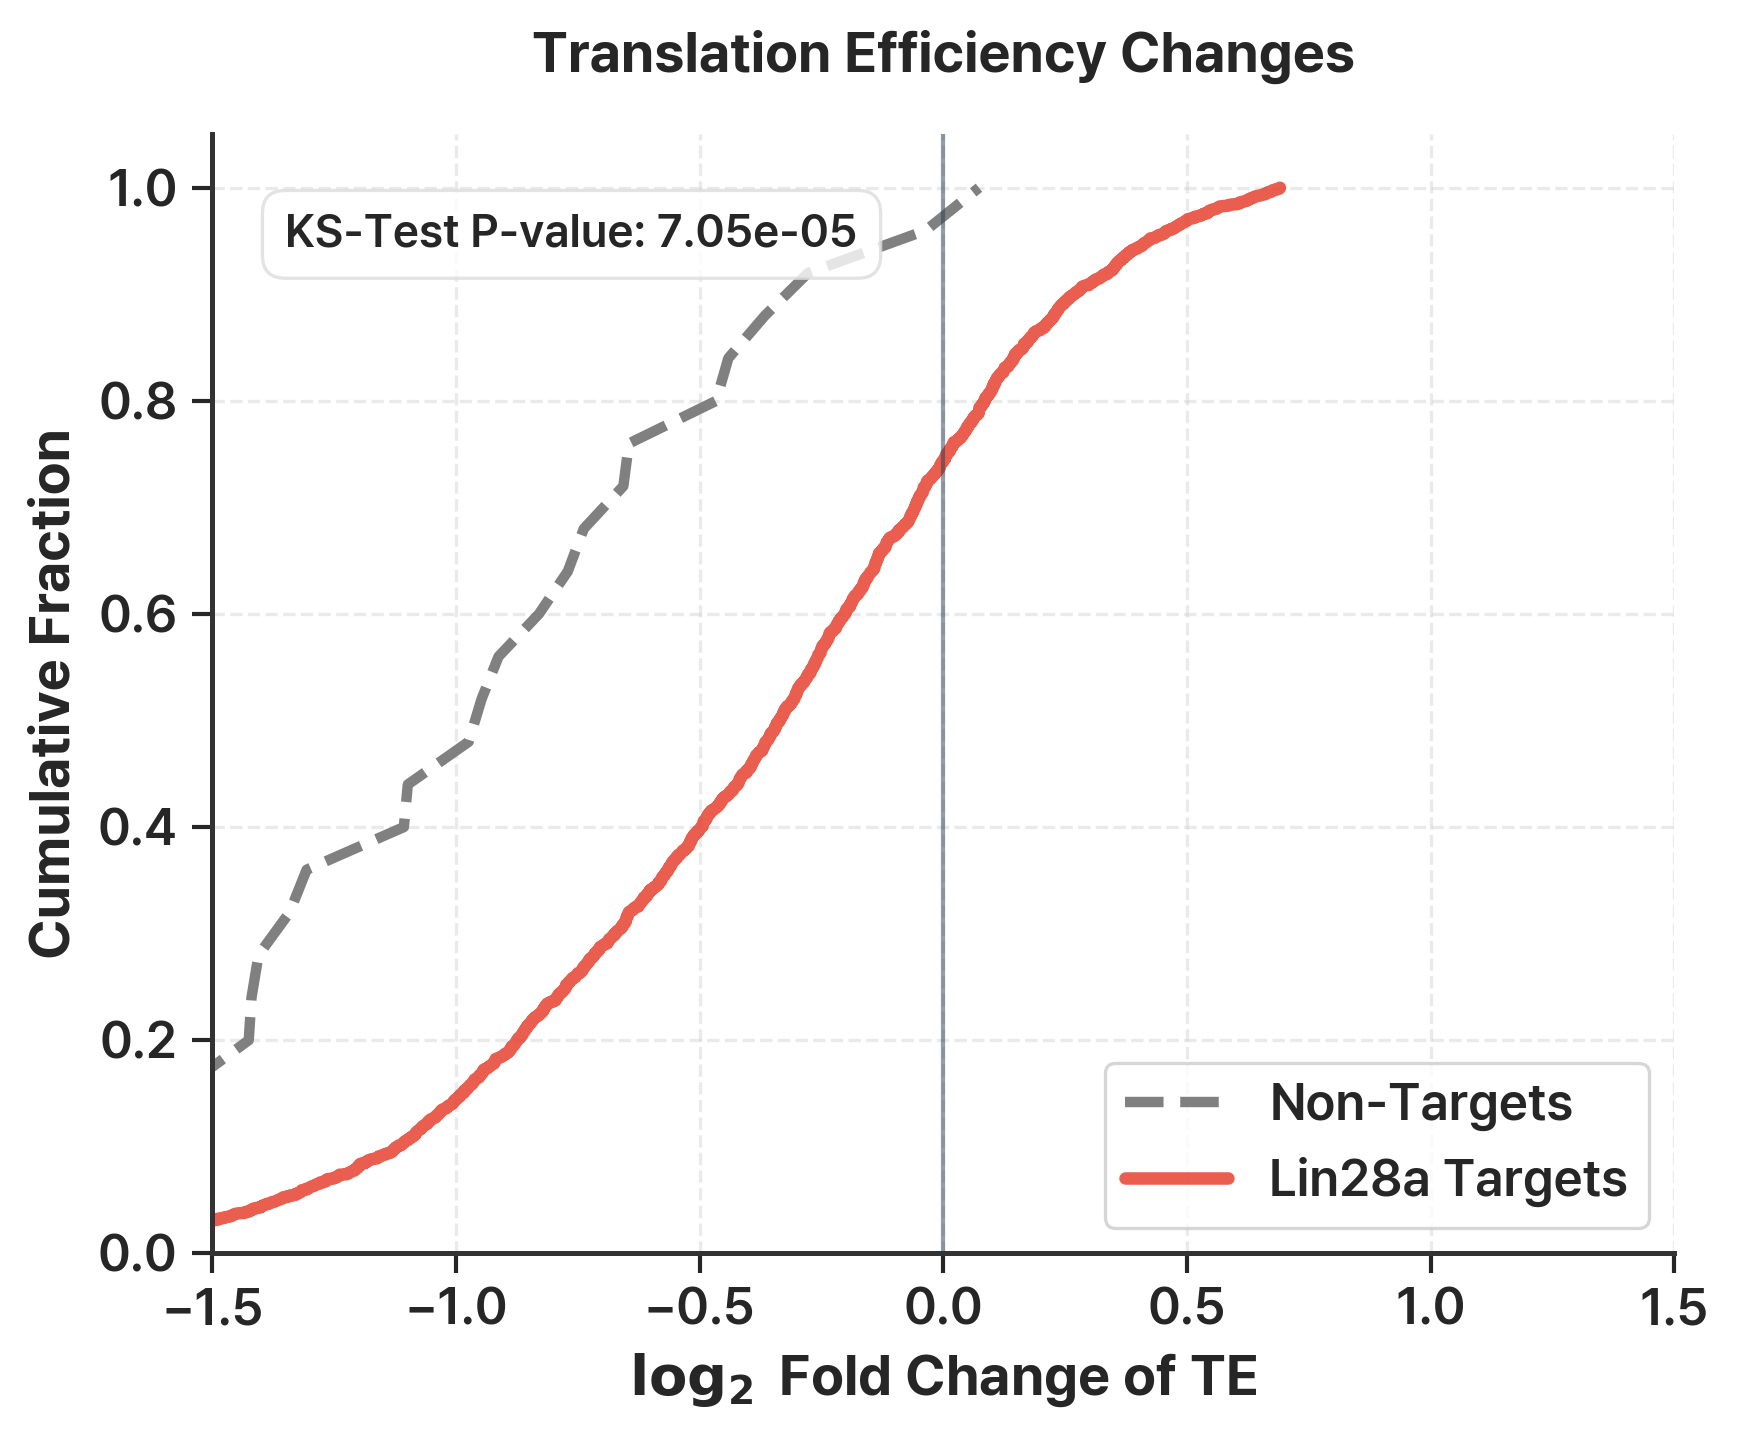
\includegraphics[width=0.6\textwidth]{report_figures_revised/Revised_Fig1_CDF.png}
    \caption{CDF Plot of Translation Efficiency Changes. Red line indicates Lin28a targets, while dashed grey line indicates non-targets.}
    \label{fig:cdf}
\end{figure}

분석 결과(Figure \ref{fig:cdf}), Lin28a Target 그룹의 $\log_2$ Fold Change of TE 분포가 Non-Target 그룹에 비해 우측으로 뚜렷하게 치우쳐 있음을 확인했다(KS-Test 통계적 유의성 확인). 이는 Lin28a가 표적 mRNA의 번역을 효과적으로 억제하고 있었으며, Knockdown을 통해 그 억제가 해제되어 번역이 촉진되었음을 정량적으로 뒷받침한다.

\clearpage
\subsection{Graded Derepression by CLIP Enrichment}
나아가 Lin28a의 억제 효과가 표적 mRNA에 대한 물리적인 결합 강도에 비례하는지 검증하였다. 표적 그룹을 결합 강도(CLIP Enrichment)에 따라 4개의 사분위수(Q1~Q4)로 세분화하여 TE 변화 양상을 비교하였다.

\begin{figure}[H]
    \centering
    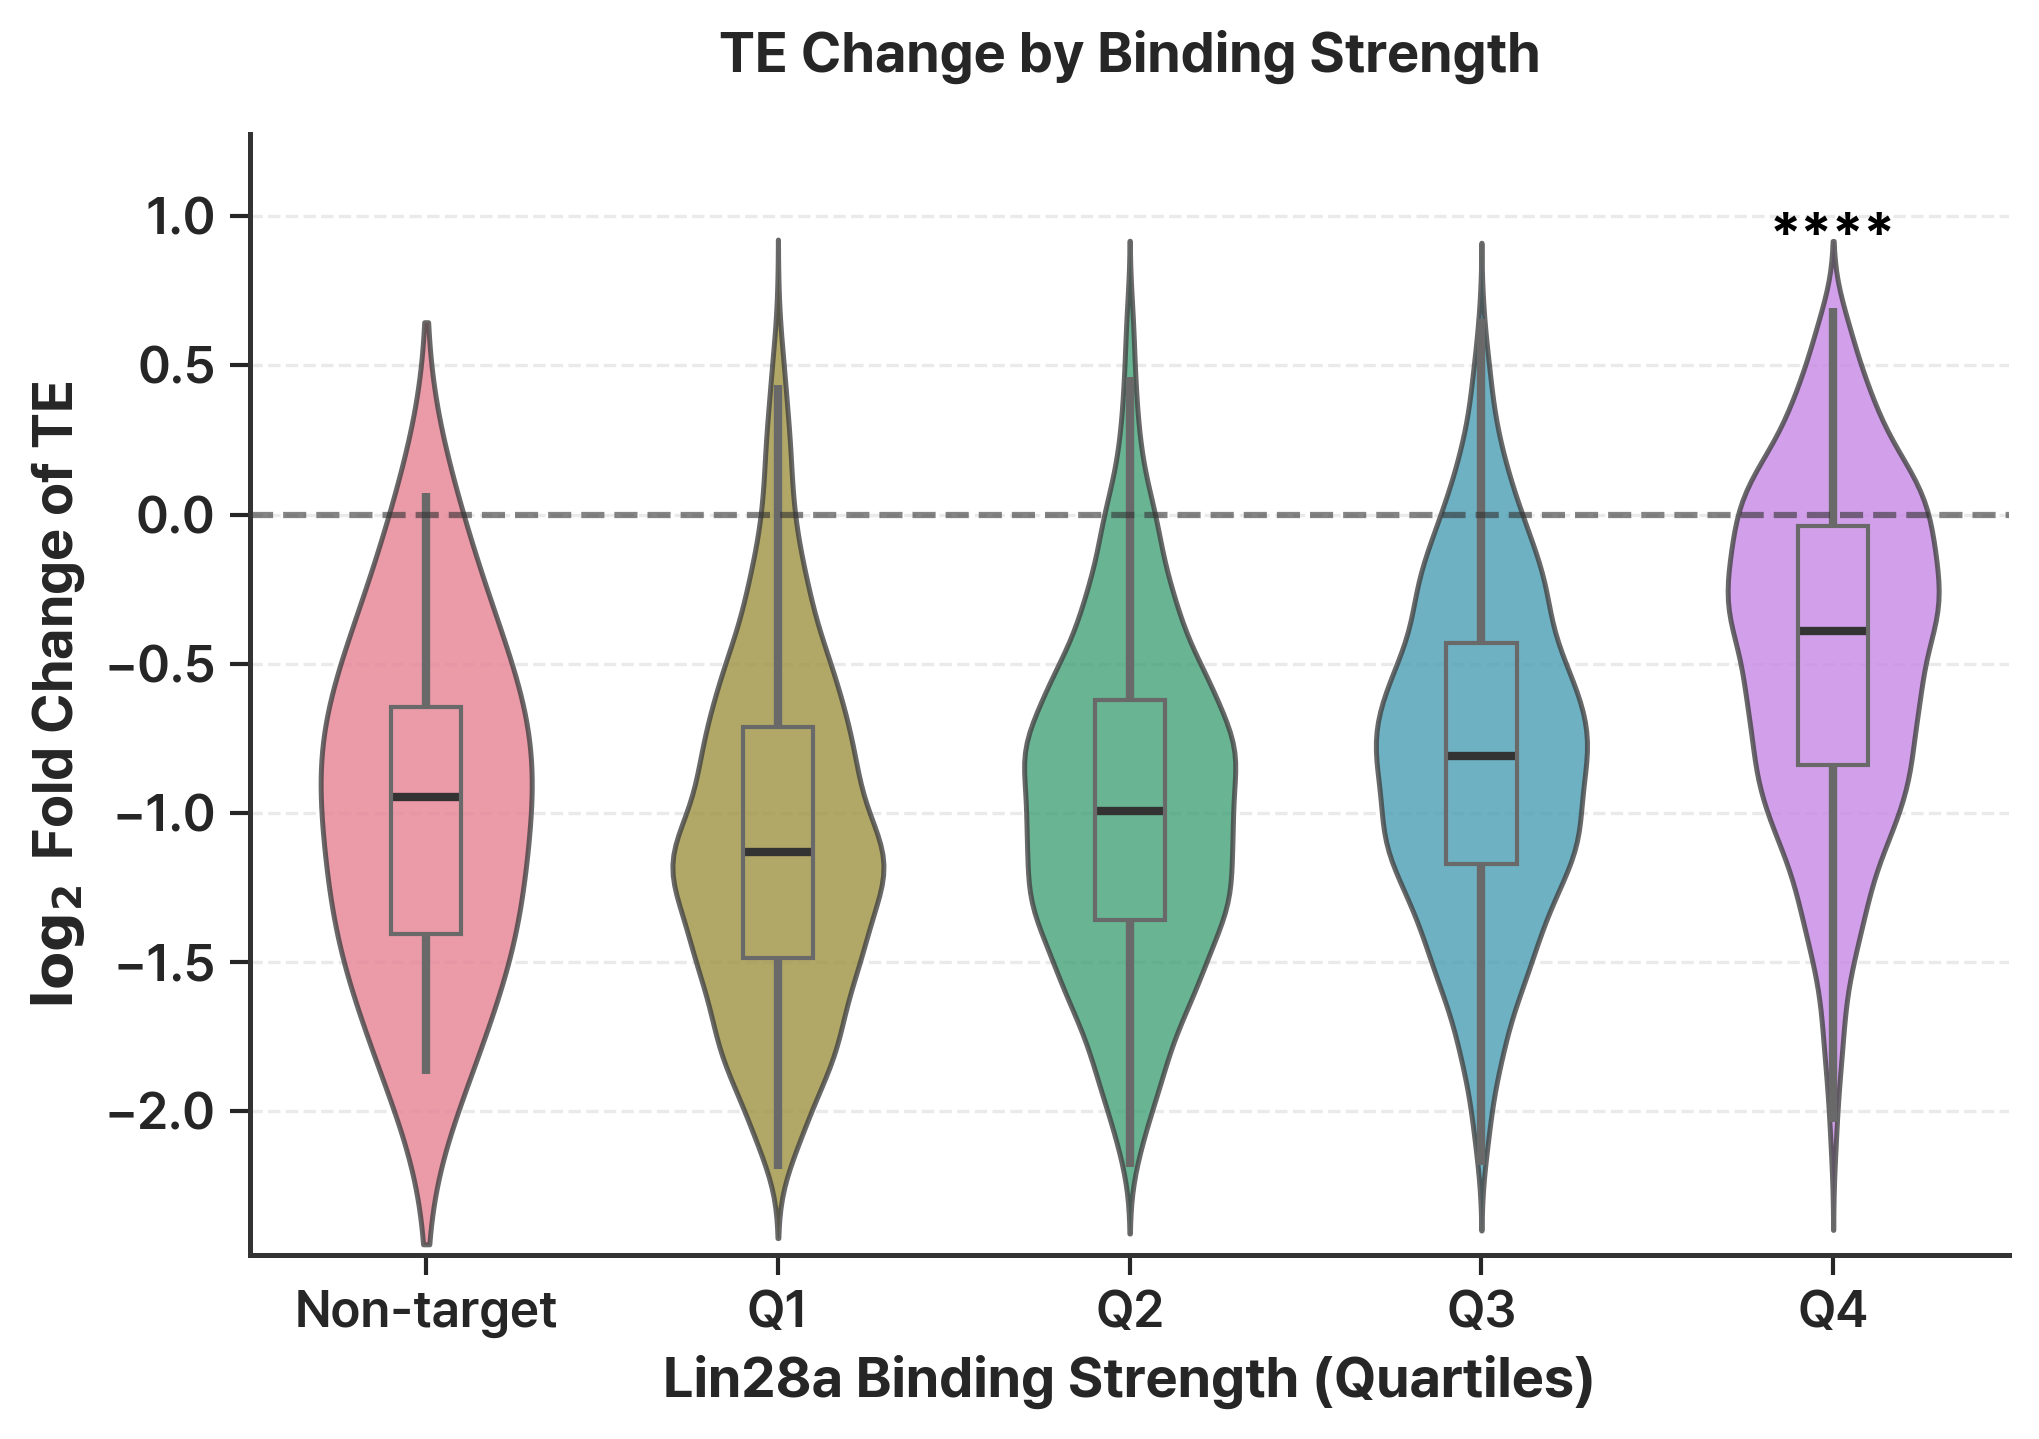
\includegraphics[width=0.65\textwidth]{report_figures_revised/Revised_Fig2_Violin_Quartiles.png}
    \caption{Violin plot of TE changes grouped by Lin28a binding strength quartiles. Statistical significance of each quartile against the non-target group is indicated by asterisks (**** p $<$ 0.0001).}
    \label{fig:violin_quartile}
\end{figure}

\begin{figure}[H]
    \centering
    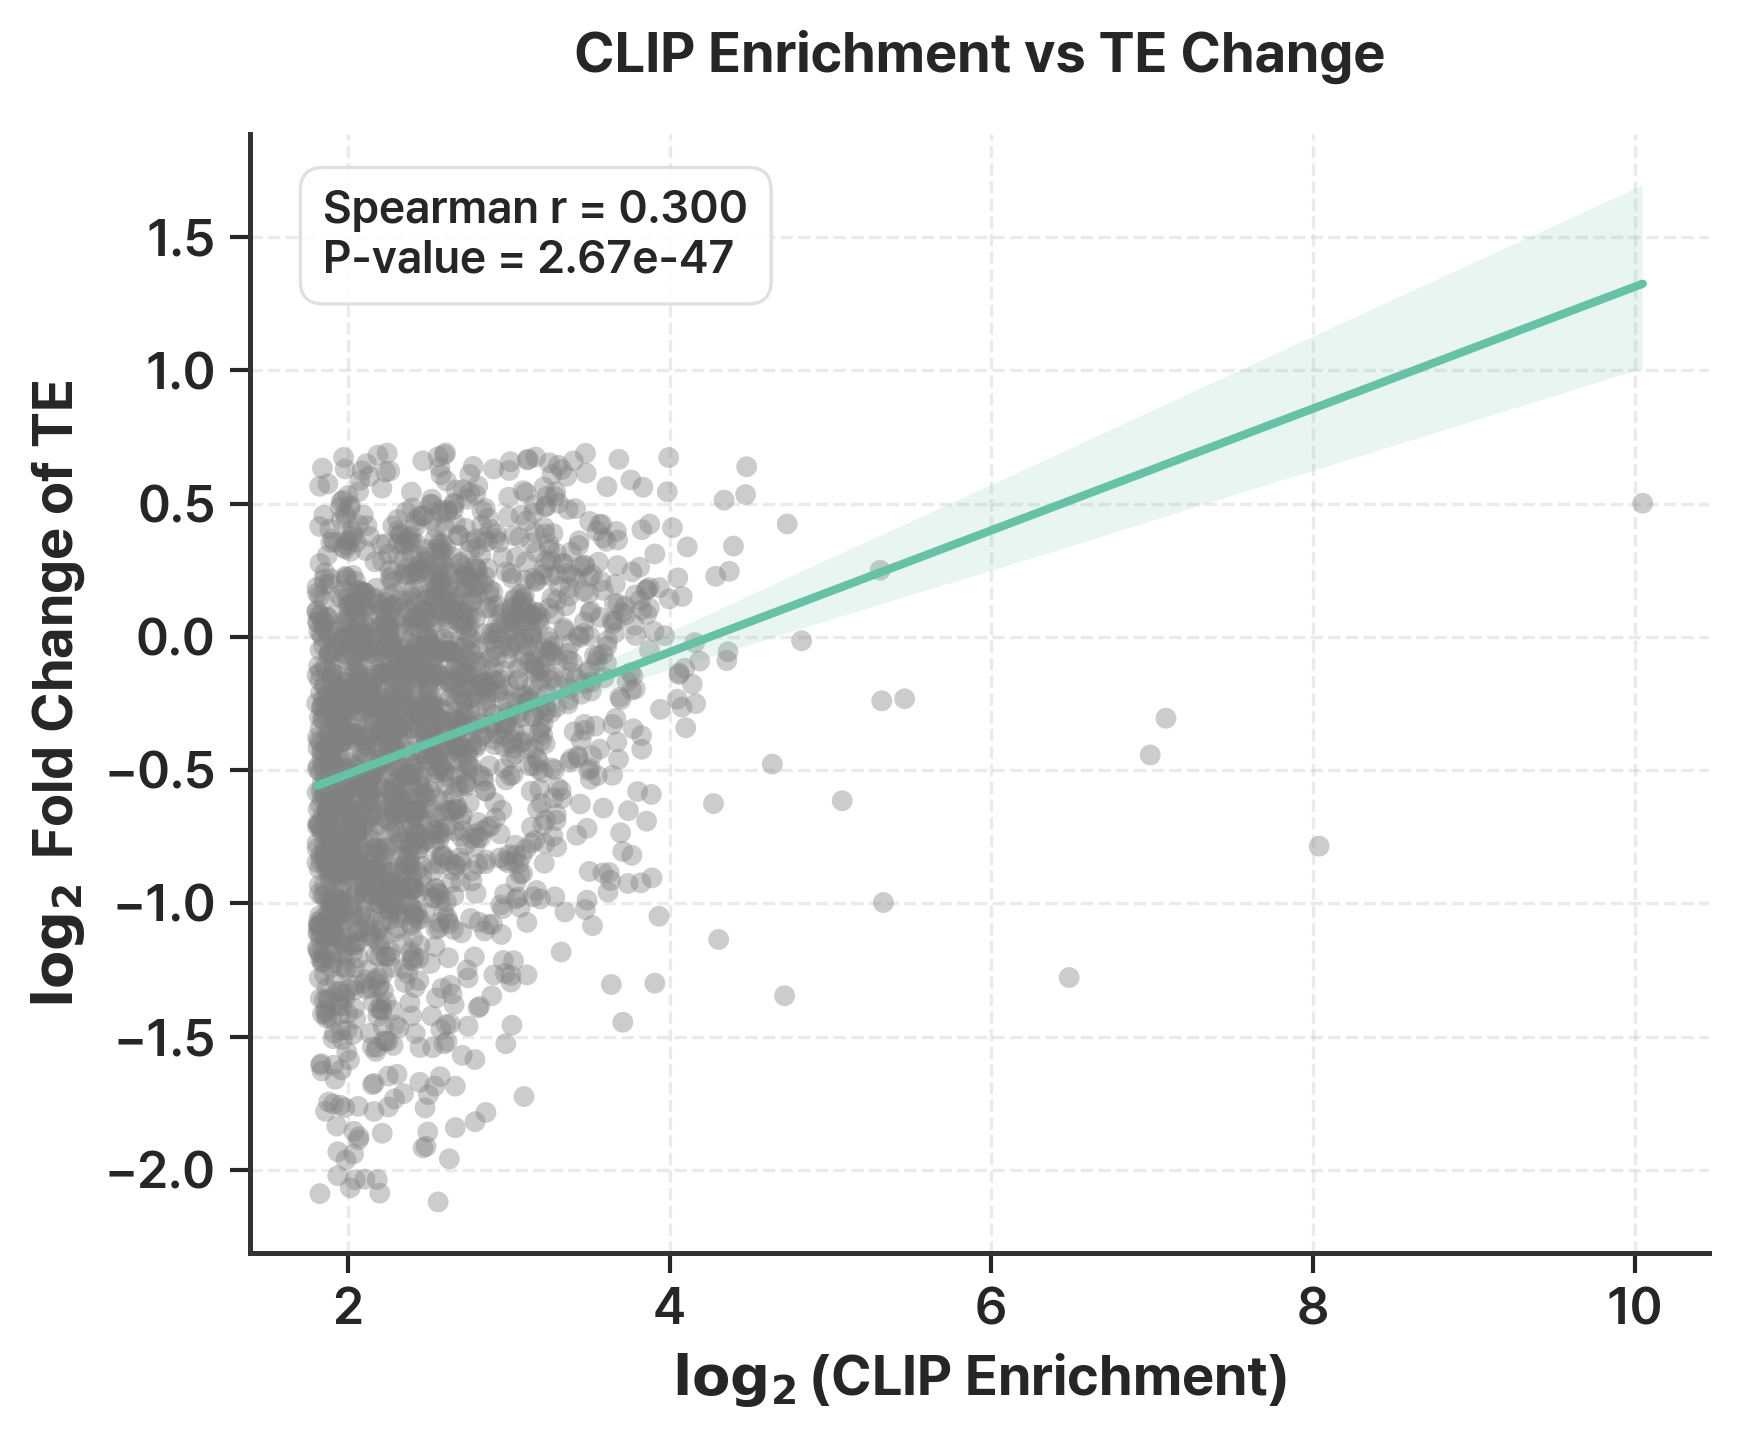
\includegraphics[width=0.55\textwidth]{report_figures_revised/Revised_Fig3_Scatter.png}
    \caption{Scatter plot showing Spearman correlation between CLIP enrichment and TE change.}
    \label{fig:scatter}
\end{figure}

Figure \ref{fig:violin_quartile}에서 볼 수 있듯, 결합 친화도가 가장 높은 Q4 그룹에서 번역 억제 해제(Derepression) 효과가 가장 강력하게 나타났으며, Kruskal-Wallis 검정 결과 그룹 간 유의미한 차이가 확인되었다. 연속형 변수로서의 상관관계를 보여주는 Figure \ref{fig:scatter}에서도 Spearman Correlation을 통해 양의 상관관계가 증명되었다. 이는 Lin28a에 의한 번역 억제가 'All-or-None' 방식이 아닌, 결합 강도에 따른 'Graded' 방식으로 조절됨을 의미한다.

\subsection{Subcellular Localization Dependency of Translational Repression}
마지막으로, Lin28a의 번역 억제가 mRNA가 번역되는 세포 내 공간이나 리보솜 복합체 종류에 따라 달라지는지를 검토하였다. 이를 위해 각 유전자의 세포 내 최종 목적지(Subcellular Localization) 정보를 병합하여 국소화 유형별 TE 변화량을 비교했다.

\begin{figure}[H]
    \centering
    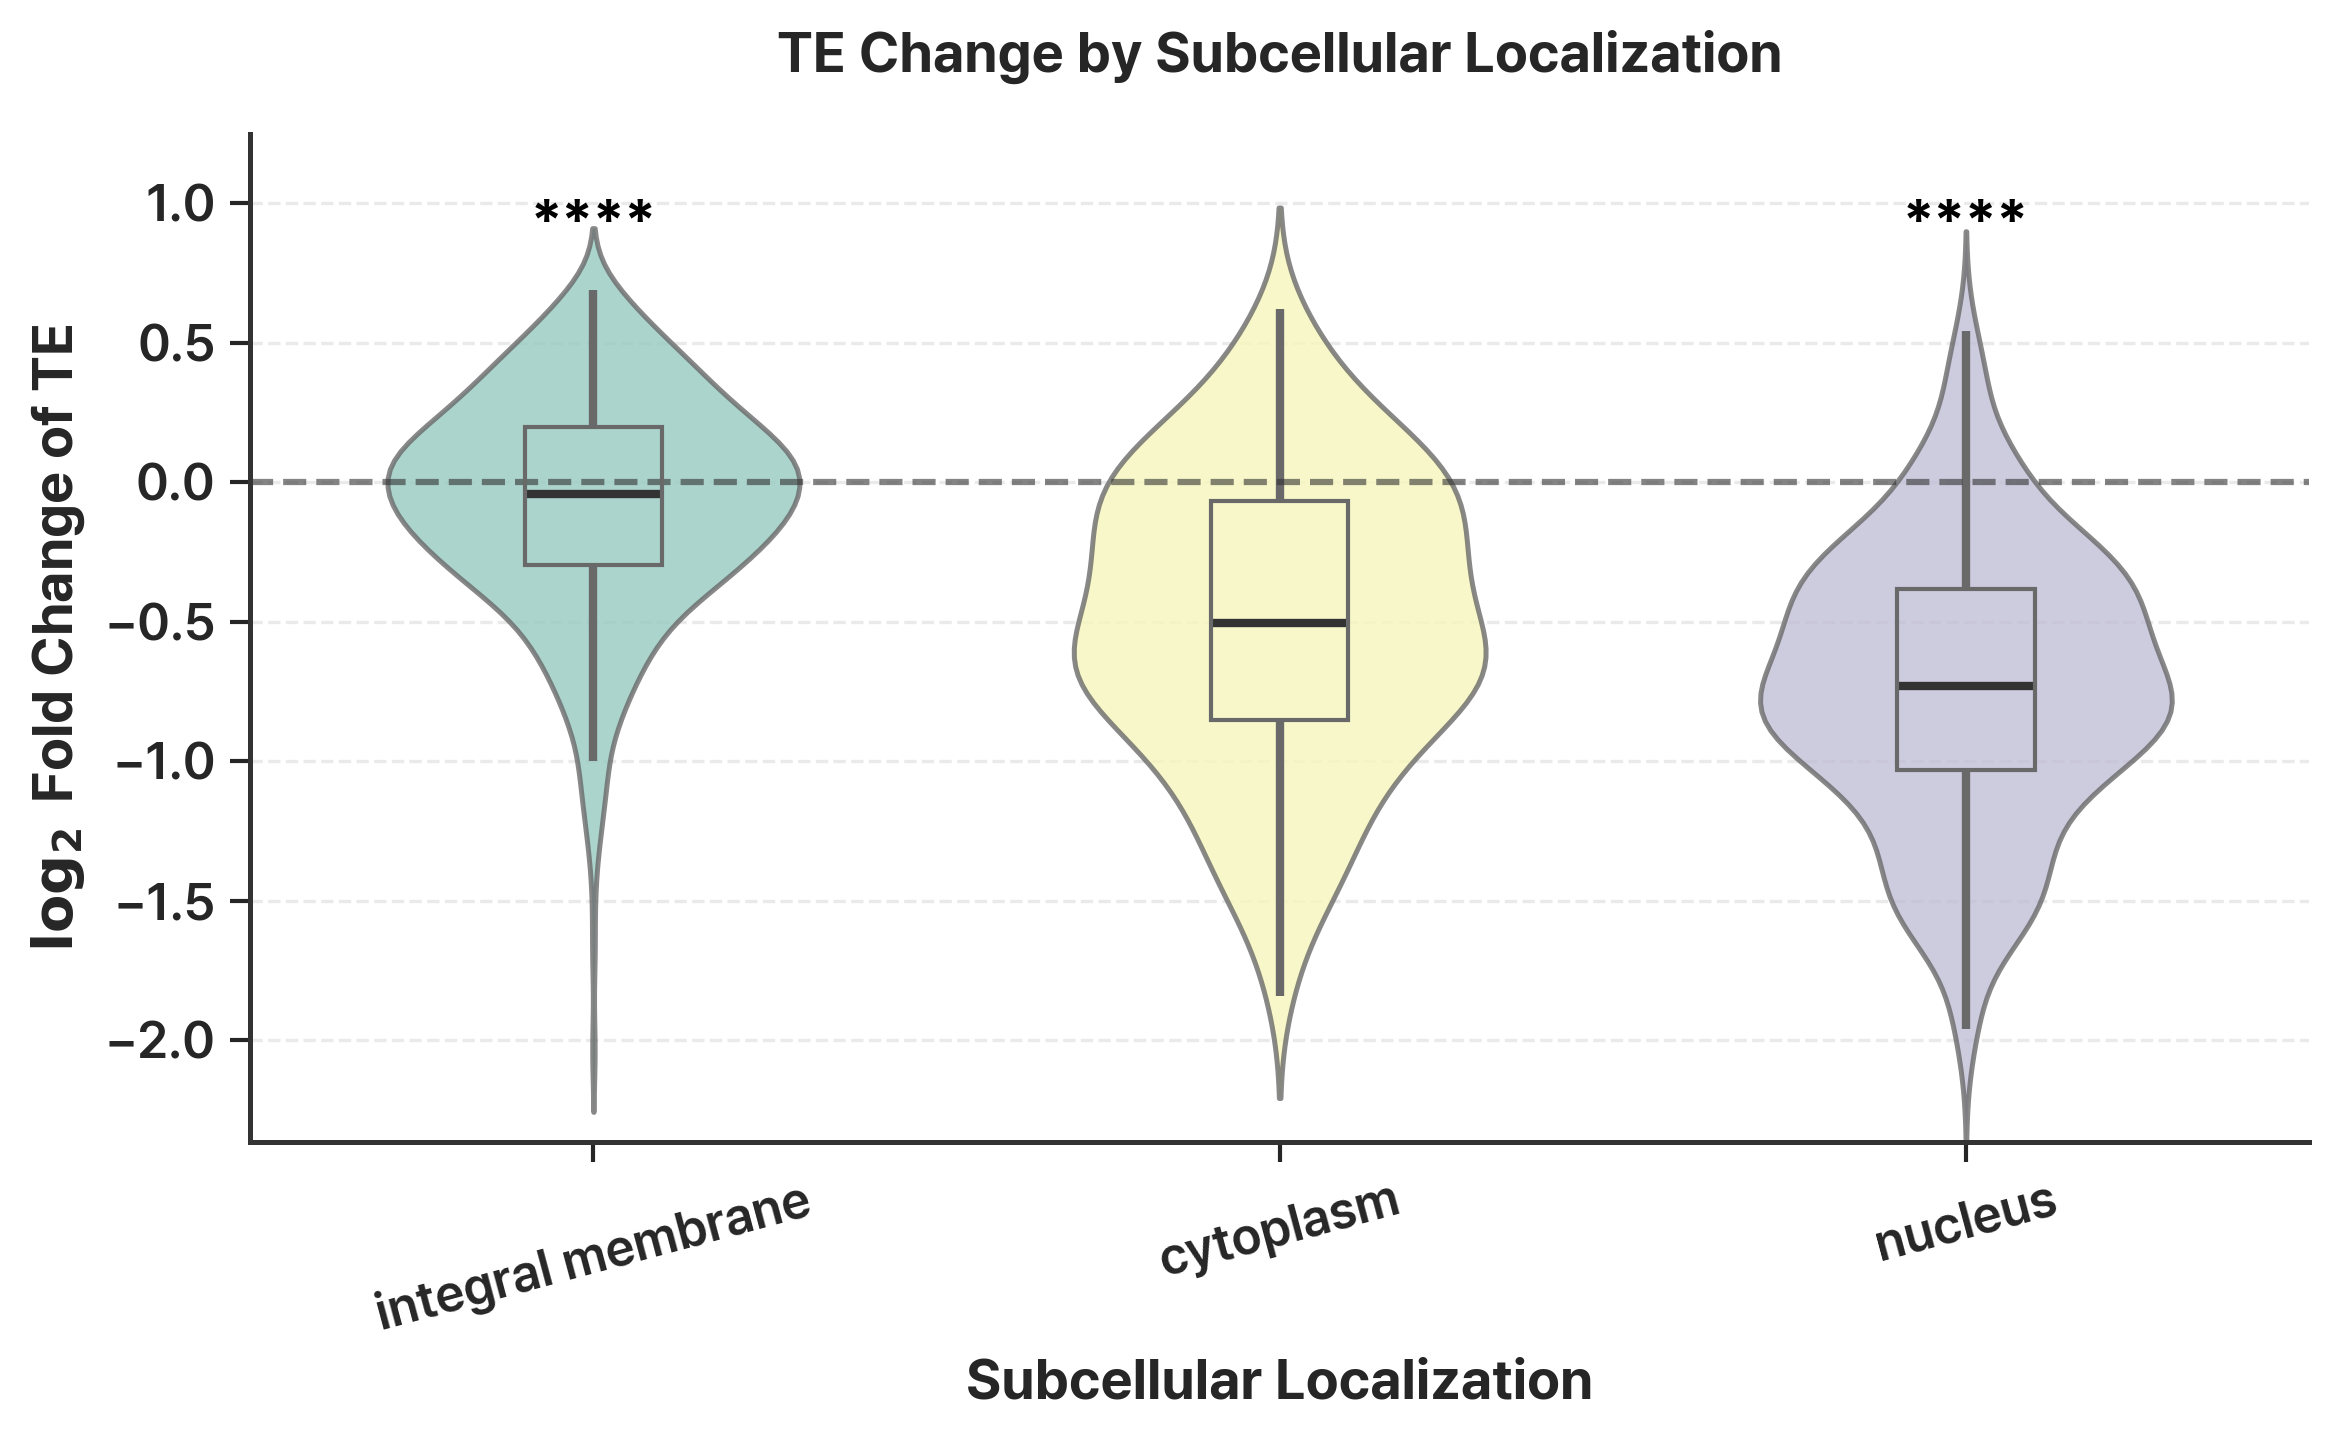
\includegraphics[width=0.8\textwidth]{report_figures_revised/Revised_Fig4_Violin_Loc.png}
    \caption{TE change of target mRNAs across various subcellular localization categories. Statistical significance compared to cytoplasm is indicated by asterisks (**** p $<$ 0.0001).}
    \label{fig:violin_loc}
\end{figure}

Figure \ref{fig:violin_loc}에 나타난 바와 같이, 세포질(Cytoplasm)로 향하는 단백질을 인코딩하는 mRNA와 내재성 막단백질(Integral membrane) 등을 인코딩하는 mRNA 간에 TE 변화 분포에서 유의미한 차이(Mann-Whitney U Test 검증)가 관찰되었다. 이는 표적 단백질 합성이 주로 일어나는 리보솜의 물리적 위치(Free ribosome vs ER-bound Ribosome)에 따라 Lin28a 단백질의 억제 효능이나 작용 기전이 상이할 수 있음을 나타낸다.

\subsection{Physical Binding Affinity Correlates with Subcellular Localization}
앞선 결과에서 Integral membrane으로 향하는 mRNA들의 번역 억제가 더 강하게 일어남을 확인하였다. 이것이 실제로 Lin28a 단백질이 해당 mRNA들에 더 자주 물리적으로 결합하기 때문인지 검증하기 위해, 국소화 유형별 CLIP Enrichment 값을 비교했다 (Figure \ref{fig:violin_clip_loc}).

\begin{figure}[H]
    \centering
    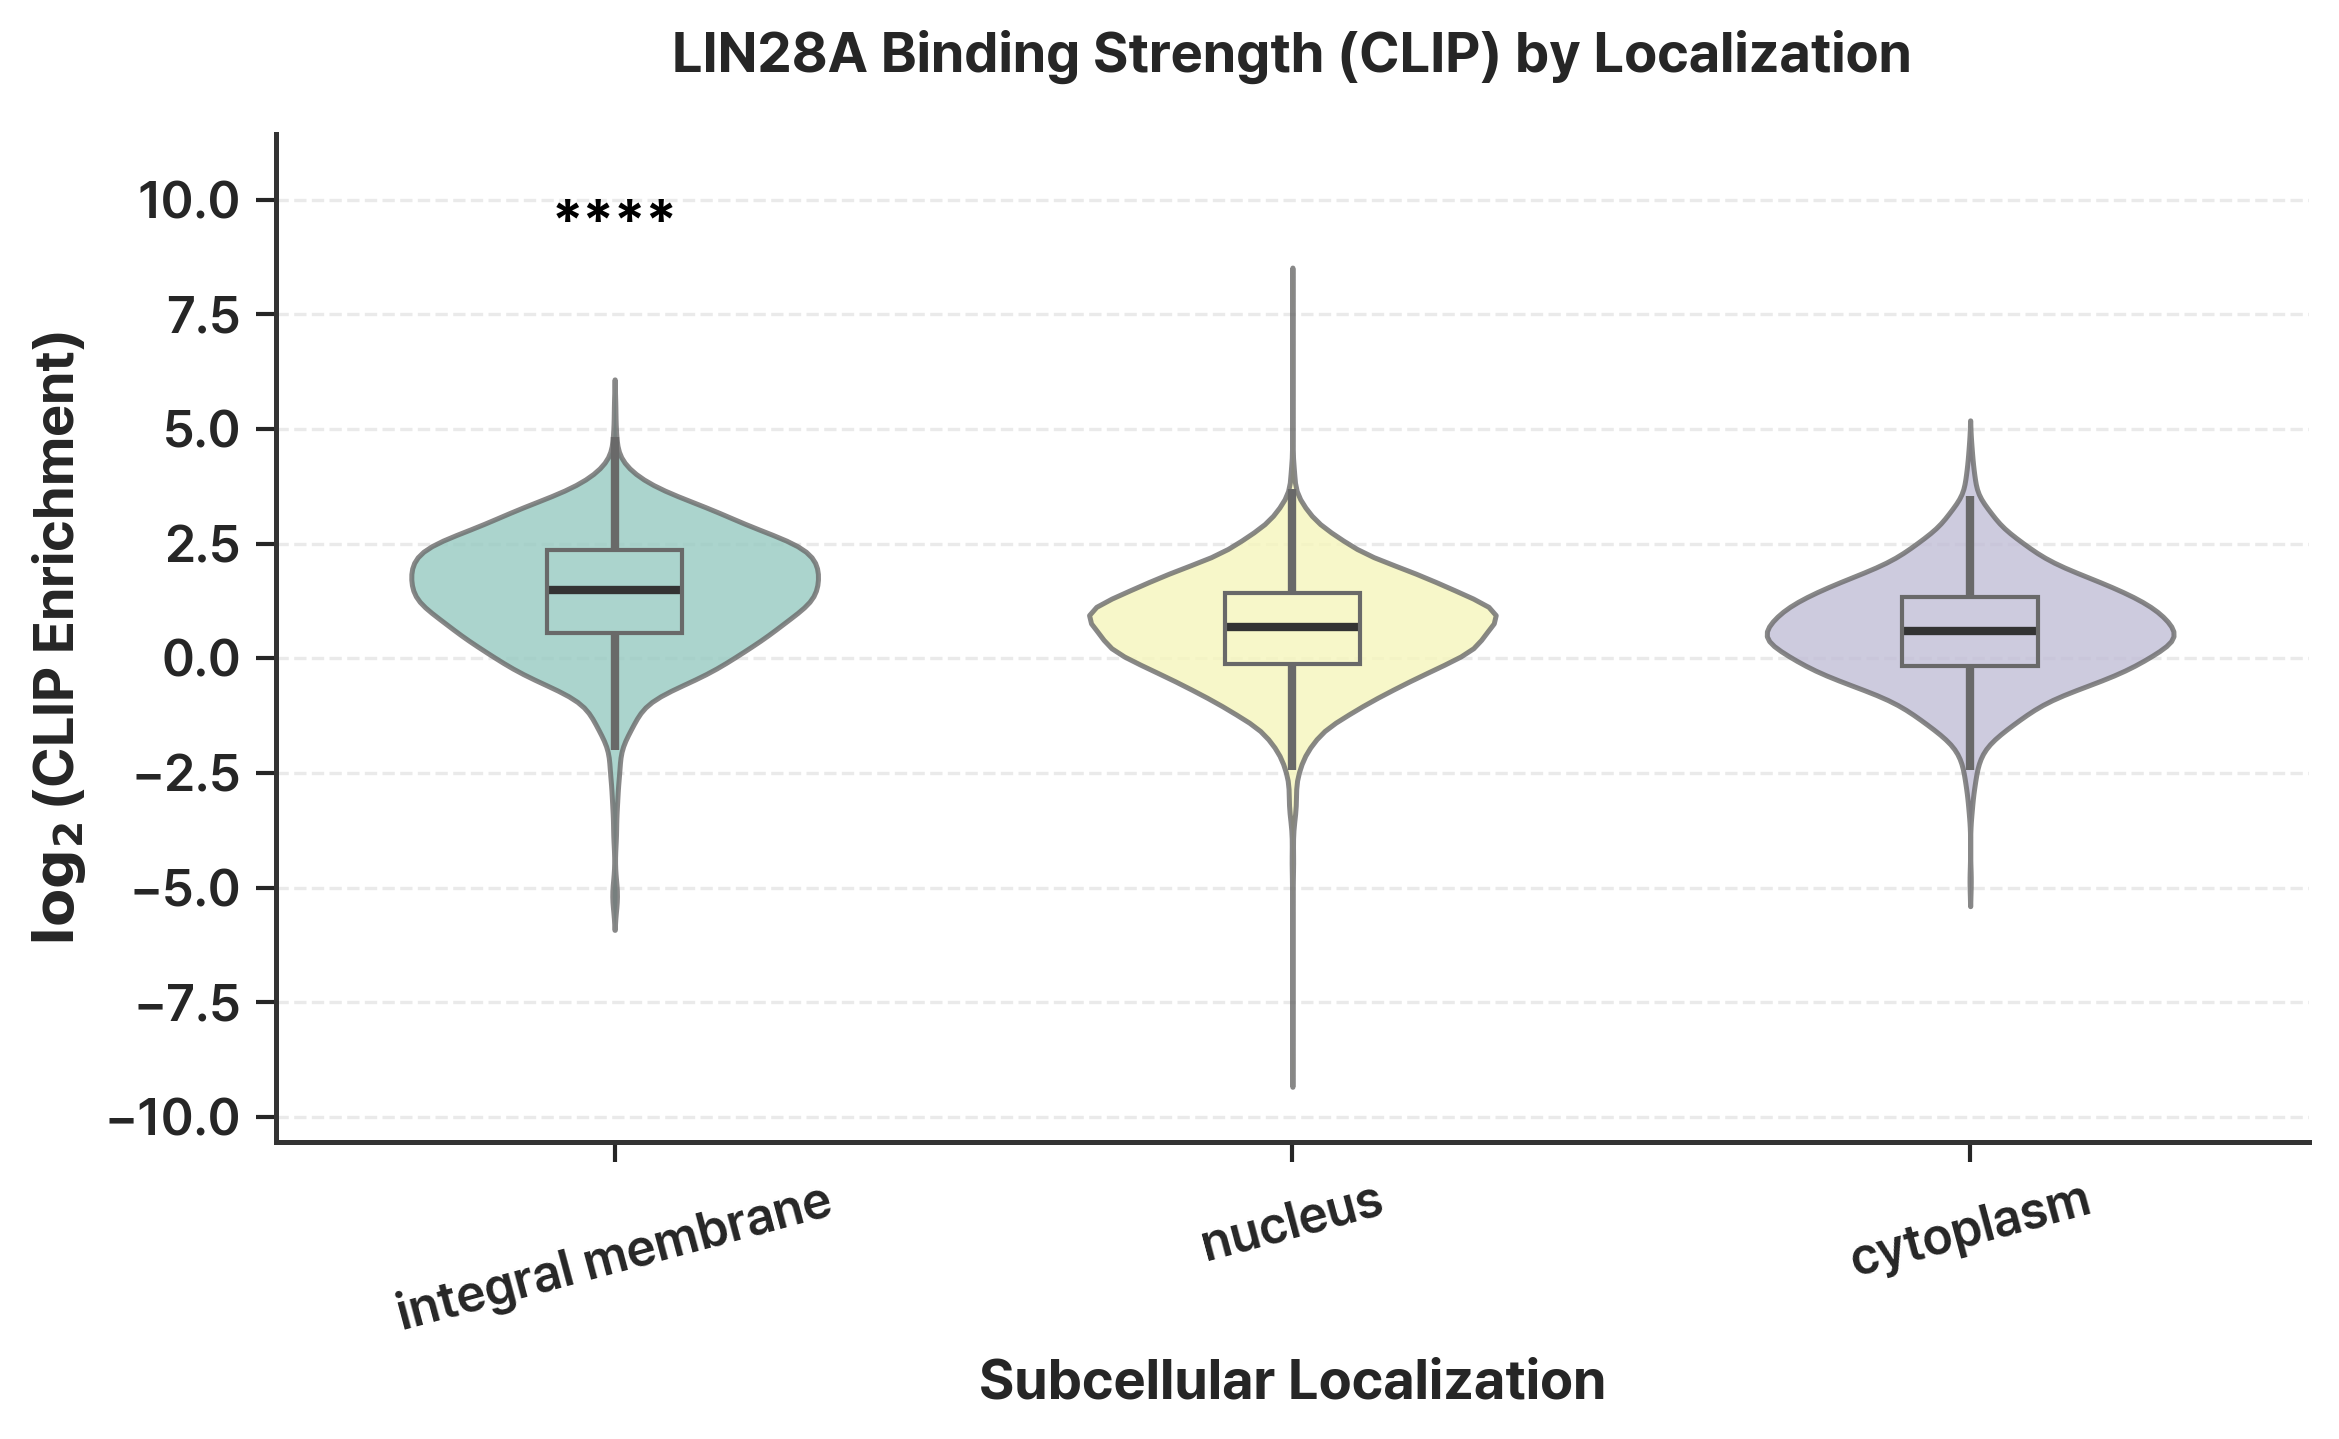
\includegraphics[width=0.8\textwidth]{report_figures_revised/Revised_Fig5_Violin_CLIP_Loc.png}
    \caption{LIN28A binding strength (CLIP enrichment) across various subcellular localization categories. Statistical significance compared to cytoplasm is indicated by asterisks.}
    \label{fig:violin_clip_loc}
\end{figure}

분석 결과, Integral membrane 단백질을 인코딩하는 mRNA들에 대한 Lin28a의 물리적 결합 빈도 및 강도(CLIP Enrichment)가 Cytoplasm 단백질 대비 유의미하게 더 높음을 확인하였다. 이는 Lin28a가 공간적으로 소포체 주변에 분포하며, ER-associated mRNA들을 선택적으로 더 많이 타겟팅하여 번역을 억제한다는 메커니즘을 강력하게 뒷받침한다.

\section{Discussion}
본 연구 결과는 Lin28a가 표적 mRNA와의 결합 친화도 및 공간적 맥락을 통합적으로 활용하여 유전자 발현을 미세 조절하는 정교한 번역 억제자(Translational repressor)임을 시사한다. 분석 결과, 억제 효과가 결합 강도(CLIP Enrichment)에 비례하는 용량 의존적(Graded) 패턴으로 나타났는데, 이는 Lin28a 단백질 농도의 미세한 변화나 결합 친화도의 차이가 표적 유전자 발현의 점진적인 튜닝을 가능하게 함을 보여준다.

또한, Subcellular Localization에 따른 분석에서 세포질(Cytoplasm) 단백질 대비 Integral membrane을 인코딩하는 mRNA들이 Lin28a와 더욱 강하게 물리적으로 결합하며, 이에 따라 번역 억제 양상 또한 상이하고 뚜렷하게 관찰되었다. 이러한 결과는 Lin28a가 소포체(ER) 주변에 위치하며 ER-bound Ribosome에서 일어나는 번역을 특이적으로 억제한다는 Cho et al. (2012)의 연구 결과와 완벽하게 부합한다 \cite{cho2012}. Lin28a는 이러한 기전을 통해 줄기세포나 초기 발생 단계에서 분비 경로(secretory pathway) 단백질의 발현을 억제함으로써 세포의 미분화 상태 유지 및 운명 결정에 기여할 것으로 보인다 \cite{hu2024, cho2012}. 결론적으로, 본 분석은 전사 후 조절 기작을 이해하는 데 있어 RNA 결합 강도뿐만 아니라 표적 mRNA의 위치적(Spatial) 맥락을 함께 고려하는 것이 필수적임을 재차 입증하였다.

\begin{thebibliography}{9}
\bibitem{heo2008} Heo I, Joo C, Cho J, Ha M, Han J, Kim VN. Lin28 mediates the terminal uridylation of let-7 precursor MicroRNA. \textit{Mol Cell.} 2008 Oct 24;32(2):276-84. doi: 10.1016/j.molcel.2008.09.014. PMID: 18951094.
\bibitem{cho2012} Cho J, Chang H, Kwon SC, Kim B, Kim Y, Choe J, Ha M, Kim YK, Kim VN. LIN28A is a suppressor of ER-associated translation in embryonic stem cells. \textit{Cell.} 2012 Nov 9;151(4):765-777. doi: 10.1016/j.cell.2012.10.019. PMID: 23102813.
\bibitem{hu2024} Hu J, Yuan J, Shi Q, Guo X, Liu L, Esteban MA, Lv Y. Single-cell profiling identifies LIN28A mRNA targets in the mouse pluripotent-to-2C-like transition and somatic cell reprogramming. \textit{J Biol Chem.} 2024 Nov;300(11):107824. doi: 10.1016/j.jbc.2024.107824. PMID: 39343008.
\end{thebibliography}

\end{document}
